\section{\trJoin{}与\trSlice{}}
\label{sec:joins-and-slices}

本节我们讨论\trSimplicialSets{}中的一个构造，它模仿普通\trCategoryTheory{}中%
\trJoin{}与\trSlice{}的概念。本节的技术风味与上一节相似，尽管其技术投入明显较少。
这里发展出的工具是\trJoyal{}提升定理（Joyal's lifting theorem）之证明的一个中心构件，
该定理将在下一章中讨论。

\begin{definition}\label{def:join-categories}
设 $\C$ 与 $\D$ 是\trCategories{}。那么\emph{\trJoin{}}（join）
$\C \star \D$ 由下述\trCategory{}给出：
\[
\mathrm{Ob}(\C \star \D) = \mathrm{Ob}(\C) \amalg \mathrm{Ob}(\D)
\]
此\trCategory{}中的 Hom 集由下式给出
\[
\mathrm{Hom}_{\C \star \D}(x, y) =
\begin{cases}
\mathrm{Hom}_{\C}(x, y) & \text{若 } x, y \in \C,\\
\mathrm{Hom}_{\D}(x, y) & \text{若 } x, y \in \D,\\
\ast & \text{若 } x \in \C,\, y \in \D,\\
\varnothing & \text{若 } x \in \D,\, y \in \C.
\end{cases}
\]
\end{definition}

\begin{remark}\label{rem:join-not-symmetric}
注意，\trJoin{}不是对称的。
\end{remark}

\begin{definition}\label{def:slice-categories}
设 $\C$ 是一个\trCategory{}，并设 $x \in \C$ 是一个\trObject{}。那么存在由 $x$
之上与 $x$ 之下的\trObject{}构成的\trCategories{} $\C_{/x}$ 与 $\C_{x/}$，称为%
\emph{\trSliceCategory{}}（slice categories）。\trObject{}由\trMorphism{}给出：
对 $\C_{/x}$ 为 $y \to x$，对 $\C_{x/}$ 为 $x \to y$。两个这类\trObject{}之间的%
\trMorphism{}由交换三角形给出。
\end{definition}

\begin{remark}\label{rem:slice-cocomplete}
若 $\C$ 是一个\trCocomplete{}（cocomplete）\trCategory{}，而 $x$ 是 $\C$ 的一个%
\trObject{}，那么由 $x$ 之下的\trObject{}构成的\trSliceCategory{} $\C_{x/}$ 仍是%
\trCocomplete{}。然而，\trForgetfulFunctor{}（forgetful functor）
$\C_{x/} \to \C$ 并不保持所有%
\trColimit{}，见\cref{lem:slice-complete}。
\end{remark}

\begin{definition}\label{def:cuts}
给定一个\trLinearlyOrderedSet{}（linearly ordered set）$J$，我们把 $J$ 的\emph{\trCut{}}%
（cut）之集记作 $\mathrm{Cut}(J)$，定义为把 $J$ 写成 $J = J_1 \amalg J_2$ 的那些
分解，即将 $J$ 分解成两个不相交的部分 $J_1$ 与 $J_2$，使得只要 $x \in J_1$ 且
$y \in J_2$，就有 $x < y$。半空\trCut{}（half-empty cut）$(\varnothing, J)$ 与
$(J, \varnothing)$ 是允许的。
\end{definition}

\begin{lemma}\label{lem:cut-pullback}
给定\trLinearlyOrderedSet{} $J$ 与 $J'$ 以及一个映射 $\alpha\colon J \to J'$，并给定
$(J_1', J_2') \in \mathrm{Cut}(J')$，那么存在唯一的\trCut{}%
$(J_1, J_2) \in \mathrm{Cut}(J)$，使得 $\alpha$ 限制为映射
$\alpha_1\colon J_1 \to J_1'$ 与 $\alpha_2\colon J_2 \to J_2'$。
\end{lemma}

\begin{proof}
我们需定义 $J_i = \alpha^{-1}(J_i')$。唯一需要检验的是这确实是 $J$ 的一个\trCut{}。
但这由 $\alpha$ 保持序这一事实得出。
\end{proof}

\begin{observation}\label{obs:cut-representable}
这一结果表明，$\mathrm{Cut}(-)$ 是从\trLinearlyOrderedSet{}到集合的一个%
\trContravariantFunctor{}（contravariant functor）。事实上，$\mathrm{Cut}(-)$
关于 $[1]$ 是\trRepresentable{}（representable）。
\end{observation}

\begin{definition}\label{def:join-simplicial-sets}
设 $X$ 与 $Y$ 是\trSimplicialSets{}。我们把它们的\trJoin{} $X \star Y$ 定义为
如下给出的\trSimplicialSet{}：对有限\trLinearlyOrderedSet{} $J$，我们令
\[
(X \star Y)(J) =
\coprod_{(J_1, J_2) \in \mathrm{Cut}(J)} X(J_1) \times Y(J_2)
\]
其中我们约定 $X(\varnothing) = \ast = Y(\varnothing)$。设 $\alpha\colon J \to J'$
是\trLinearlyOrderedSet{}的一个\trMorphism{}，并考虑 $J'$ 的一个\trCut{}。那么对于如%
\cref{lem:cut-pullback} 中那般与之相伴的 $J$ 的\trCut{}，存在映射
\[
X(J_1') \times Y(J_2') \to X(J_1) \times Y(J_2).
\]
这提供一个唯一的映射
\[
(X \star Y)(J') \to (X \star Y)(J)
\]
它在 $J'$ 的每个\trCut{}上限制为上述映射，从而使 $X \star Y$ 成为一个%
\trSimplicialSet{}。
\end{definition}

\begin{example*}
给定两个普通\trCategories{} $\C$ 与 $\D$，我们有
\[
\mathrm{N}(\C \star \D) \cong \mathrm{N}(\C) \star \mathrm{N}(\D).
\]
特别地，$\Delta^n \star \Delta^m = \Delta^{n+1+m}$ 成立。为了证明这一断言，我们
构造一个\trSimplicialMap{}%
\[
\mathrm{N}(\C \star \D) \to \mathrm{N}(\C) \star \mathrm{N}(\D)
\]
其做法是注意到 $\mathrm{N}(\C \star \D)$ 中任何 $n$-\trSimplex{}都确定
$[n]$ 的一个\trCut{}：在某个点处，人们从 $\C$ 中的\trMorphism{}跳到 $\D$ 中的%
\trMorphism{}。容易看出，这个映射是同构。
\end{example*}

\begin{lemma}\label{lem:join-functor}
给定一个\trSimplicialSet{} $X$，\trJoin{}构造确定一个\trFunctor{}%
$X \star -\colon \mathrm{sSet} \to \mathrm{sSet}_{X/}$。同样地，它给出一个%
\trFunctor{} $- \star X\colon \mathrm{sSet} \to \mathrm{sSet}_{X/}$。
\end{lemma}

\begin{proof}
我们需要证明：对每个 $Y \in \mathrm{sSet}$，\trSimplicialSet{} $X \star Y$ 配有
一个映射 $X \to X \star Y$。由右半空\trCut{}包含
\[
X(J) \times Y(\varnothing) \subseteq
\coprod_{(J_1, J_2) \in \mathrm{Cut}(J)} X(J_1) \times Y(J_2)
= (X \star Y)(J)
\]
这显然成立。此外，给定\trSimplicialSets{}的一个\trMorphism{} $Y \to Y'$，我们
立即看出典范图表
\begin{center}
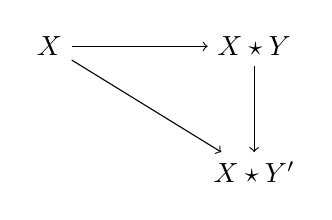
\begin{tikzpicture}
  \node (x) at (0,0) {$X$};
  \node (xy) at (2.6,0) {$X \star Y$};
  \node (xyy) at (2.6,-1.6) {$X \star Y'$};
  \draw[->] (x) -- (xy);
  \draw[->] (xy) -- (xyy);
  \draw[->] (x) -- (xyy);
\end{tikzpicture}
\end{center}
交换，且\trFunctor{}性也是显然的。
\end{proof}

\begin{lemma}\label{lem:factorization-over-delta-1}
设 $K$ 是一个配有映射 $p\colon K \to \Delta^1$ 的\trSimplicialSet{}。那么存在一个%
\trFunctor{}性的分解，使之成为复合
\[
K \to K_0 \star K_1 \xrightarrow{\ c\ } \Delta^1,
\]
其中 $K_i = p^{-1}(i)$，而映射 $c$ 是映射
$K_0 \star K_1 \to \Delta^0 \star \Delta^0 \cong \Delta^1$。
\end{lemma}

\begin{proof}
我们需要构造映射 $K \to K_0 \star K_1$。对任意 $n \ge 0$，我们有
\[
\mathrm{Hom}_{\mathrm{sSet}}(\Delta^n, \Delta^1)
= \mathrm{Hom}([n], [1]) = \mathrm{Cut}([n]).
\]
于是，对每个 $n$-\trSimplex{} $x\colon \Delta^n \to K$，复合
$px\colon \Delta^n \to K \to \Delta^1$ 确定一个\trCut{}%
$([i], [j]) \in \mathrm{Cut}([n])$，也就是说，映射 $px\colon [n] \to [1]$ 把前
$i$ 个点送到 $0$，而把其余的点送到 $1$。由定义，这确定
$K_0([i]) \times K_1([j])$ 的一个点，后者又确定 $K_0 \star K_1$ 的一个
$n$-\trSimplex{}。

容易看出，这事实上确定了一个\trSimplicialMap{} $K \to K_0 \star K_1$，而且这个构造在
$\mathrm{sSet}_{/\Delta^1}$ 中是\trFunctor{}性的。具体地，对于交换三角形
\begin{center}
\begin{tikzpicture}
  \node (k) at (0,0) {$K$};
  \node (d) at (2.2,0) {$\Delta^1$};
  \node (kp) at (0,-1.6) {$K'$};
  \draw[->] (k) -- (d);
  \draw[->] (k) -- (kp);
  \draw[->] (kp) -- (d);
\end{tikzpicture}
\end{center}
诱导出的图表
\begin{center}
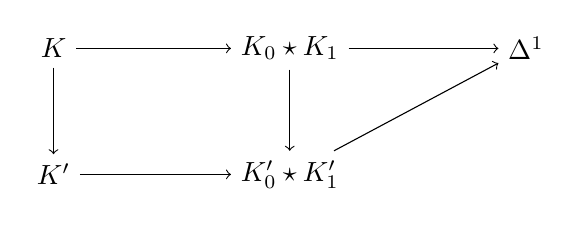
\begin{tikzpicture}
  \node (k) at (0,0) {$K$};
  \node (m) at (3,0) {$K_0 \star K_1$};
  \node (d) at (6,0) {$\Delta^1$};
  \node (kp) at (0,-1.6) {$K'$};
  \node (mp) at (3,-1.6) {$K_0' \star K_1'$};
  \draw[->] (k) -- (m);
  \draw[->] (m) -- (d);
  \draw[->] (k) -- (kp);
  \draw[->] (m) -- (mp);
  \draw[->] (kp) -- (mp);
  \draw[->] (mp) -- (d);
\end{tikzpicture}
\end{center}
也交换。
\end{proof}

\begin{corollary}\label{cor:join-factorization}
给定 $\Delta^1$ 之上的一个映射 $\varphi\colon K \to X \star Y$，即
$\mathrm{sSet}_{/\Delta^1}$ 中的一个\trMorphism{}，存在一个分解
\[
K \to K_0 \star K_1 \xrightarrow{\ f \star g\ } X \star Y.
\]
\end{corollary}

\begin{proof}
我们观察到，\cref{lem:factorization-over-delta-1} 为映射 $X \star Y \to \Delta^1$
提供的分解由 $X \star Y \to X \star Y \to \Delta^1$ 给出。由于这个分解是%
\trFunctor{}性的，我们得到一个交换图表
\begin{center}
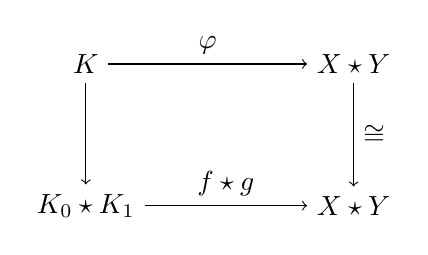
\begin{tikzpicture}
  \node (k) at (0,0) {$K$};
  \node (xy) at (3.4,0) {$X \star Y$};
  \node (m) at (0,-1.8) {$K_0 \star K_1$};
  \node (xy2) at (3.4,-1.8) {$X \star Y$};
  \draw[->] (k) -- node[above] {$\varphi$} (xy);
  \draw[->] (k) -- (m);
  \draw[->] (m) -- node[above] {$f \star g$} (xy2);
  \draw[->] (xy) -- node[right] {$\cong$} (xy2);
\end{tikzpicture}
\end{center}
断言随之得证。
\end{proof}

\begin{proposition}\label{prop:join-infinity-categories}
$X$ 与 $Y$ 是∞-\trCategories{}，当且仅当 $X \star Y$ 是一个∞-\trCategory{}。
\end{proposition}

\begin{proof}
考虑一个映射
\[
\Lambda^n_j \to X \star Y
\]
其中 $n \ge 2$ 且 $0 < j < n$。我们要证明这个映射可以扩张到 $\Delta^n$ 上。我们
可以把该映射与典范映射 $X \star Y \to \Delta^1$ 作后合成，从而得到一个分解
\[
\Lambda^n_j \to (\Lambda^n_j)_0 \star (\Lambda^n_j)_1 \to X \star Y.
\]
第一个映射有几种可能的情形。首先回忆，任何映射 $\Lambda^n_j \to \Delta^1$ 都唯一地
在 $\Delta^n$ 上分解（因为 $\Delta^1$ 是一个\trCategory{}的\trNerve{}，而
$\Lambda^n_j$ 是一个内\trHorn{}）。有三种情形需要考虑：
\begin{enumerate}[label=(\arabic*)]
  \item 映射 $\Lambda^n_j \to \Delta^1$ 在 $0$ 处取常值；
  \item 映射 $\Lambda^n_j \to \Delta^1$ 在 $1$ 处取常值；
  \item 映射 $\Lambda^n_j \to \Delta^1$ 不取常值。
\end{enumerate}
在第一种情形，我们发现映射 $\Lambda^n_j \to X \star Y$ 穿过 $X \to X \star Y$，
因此它可以扩张到 $\Delta^n$ 上当且仅当 $X$ 是一个∞-\trCategory{}：若复合
\[
\Lambda^n_j \to X \to X \star Y
\]
到 $\Delta^n$ 的一个扩张存在，则复合 $\Delta^n \to X \star Y \to \Delta^1$ 在
$0$ 处取常值，于是映射 $\Delta^n \to X \star Y$ 事实上穿过包含
$X \to X \star Y$。类似地，在第二种情形，我们发现映射
$\Lambda^n_j \to X \star Y$ 穿过 $Y \to X \star Y$，从而它可以扩张到
$\Delta^n$ 上当且仅当 $Y$ 是一个∞-\trCategory{}。

最后，让我们考虑映射 $\Lambda^n_j \to \Delta^1$ 不取常值的情形。注意，这个映射
唯一地穿过一个不取常值的映射 $\Delta^n \to \Delta^1$。不取常值的映射恰好对应于
$[n]$ 的非半空\trCut{}，于是存在 $0 \le k < n$，使得映射 $\Delta^n \to \Delta^1$
同构于典范映射 $\Delta^k \star \Delta^\ell \to \Delta^1$。由此得出，
$(\Lambda^n_j)_0$ 由 $\Lambda^n_j$ 的那些 $m$-\trSimplex{}组成，这些\trSimplex{}由映射
$[m] \to [n]$ 表示，其像含于 $\{0, \dotsc, k\}$ 之中（从而落在 $0$ 之上的纤维
里），并且存在一个异于 $j$ 的数不在 $[m] \to [n]$ 的像中（从而落在\trHorn{}%
之中）。由于 $k < n$，我们可以确定：$n$ 不在表示 $(\Lambda^n_j)_0$ 的一个
$m$-\trSimplex{} 的映射 $[m] \to [n]$ 的像中。换言之，我们发现
$(\Lambda^n_j)_0 \cong \Delta^k$。同样地，我们发现
$(\Lambda^n_j)_1 \cong \Delta^\ell$。于是\cref{cor:join-factorization} 的分解便读作
\[
\Lambda^n_j \to \Delta^k \star \Delta^\ell \to X \star Y,
\]
这正是所需的扩张。命题的证明随之轻易得出。
\end{proof}

现在，我们来到∞-\trCategories{}的\trSliceCategory{}的构造。为此，我们观察到，
若\trFunctor{} $S \star -\colon \mathrm{sSet} \to \mathrm{sSet}_{S/}$ 容许一个%
\trRightAdjoint{} $\mathrm{sSet}_{S/} \to \mathrm{sSet}$，
\[
(p\colon S \to X) \mapsto X_{p/},
\]
那么我们便得到：从 $Y$ 到 $X_{p/}$ 的一个映射，与 $\mathrm{sSet}_{S/}$ 中一个
映射 $S \star Y \to X$ 是同一回事。将这个结果特殊化到 $Y = \Delta^n$，我们便
得到一个\trSimplicialSet{}。

\begin{definition}\label{def:slice-simplicial-set}
对 $p\colon S \to X$，关联
$n \mapsto \mathrm{Hom}_{\mathrm{sSet}_{S/}}(S \star \Delta^n, X)$ 确定一个%
\trSimplicialSet{}，我们称之为 $X_{p/}$。
\end{definition}

\begin{lemma}\label{lem:slice-complete}
若一个普通\trCategory{} $\C$ 是\trComplete{}/\trCocomplete{}（(co)complete），
且 $x \in \C$ 是一个\trObject{}，那么 $\C_{x/}$ 与 $\C_{/x}$ 也是%
\trComplete{}/\trCocomplete{}。遗忘映射
$\C_{x/} \to \C$ 保持\trLimit{}与\trConnected{}\trColimit{}（即以%
\trConnected{}\trCategories{}为指标的\trColimit{}），而遗忘映射
$\C_{/x} \to \C$ 同样保持\trColimit{}与\trConnected{}\trLimit{}。
\end{lemma}

\begin{proof}
我们首先观察到 $\C_{/x} \cong (\C^{\mathrm{op}}_{x/})^{\mathrm{op}}$，因此只需
处理\trColimit{}的情形。首先，我们证明遗忘映射 $\C_{/x} \to \C$ 保持%
\trColimit{}。为此，考虑一个图表 $F\colon I \to \C_{/x}$。底图表
$I \to \C_{/x} \to \C$ 的\trColimit{}典范地带有一个到 $x$ 的映射，且容易看出，
这就产生 $F$ 的一个\trColimit{}。

图表 $F\colon I \to \C_{x/}$ 取\trColimit{}的情形则稍稍复杂一些。注意，任何这样
的图表都等价于一个图表 $G\colon I^{\triangleleft} \to \C$，其在\trCone{}点上的限制由%
\trObject{} $x$ 给出。我们观察到，存在典范\trFunctor{}%
$\Delta^0 \to I^{\triangleleft} \leftarrow I$，它们都是包含。特别地，我们有
一个典范映射
\[
x = \operatorname{colim}_{\Delta^0} G|_{\Delta^0} \to
\operatorname{colim}_{I^{\triangleleft}} G.
\]
我们断言，这个态射是 $F$ 的一个\trColimit{}。为了证明这个断言，设给定一个%
\trFunctor{} $\bar{F}\colon I^{\triangleright} \to \C_{x/}$，也就是说，在
$\C_{x/}$ 中一族彼此相容的映射 $F(i) \to (x \to y)$。我们希望证明，存在一个
唯一的映射
\[
\operatorname{colim}_{I^{\triangleleft}} G \to y
\]
它与从 $x$ 出发的两个映射都相容。由观察 $G|_I = F$，这一点便一目了然：于是对
$i \in I$，存在典范映射 $G(i) = F(i) \to y$；而对\trCone{}点，我们有 $G(\ast) = x$，
从而同样存在一个到 $y$ 的典范映射。这些映射是相容的，因为 $F$ 取值于%
\trSliceCategory{} $\C_{x/}$ 之中。这表明 $F$ 容许一个\trColimit{}，也就是上述
映射
\[
x \to \operatorname{colim}_{I^{\triangleleft}} G.
\]

为了完成本引理的证明，我们还需证明：若 $I$ 是\trConnected{}的，则典范映射
\[
\operatorname{colim}_{I} F \to
\operatorname{colim}_{I^{\triangleleft}} G
\]
是一个同构，从而\trFunctor{} $\C_{x/} \to \C$ 保持\trConnected{}\trColimit{}。我们先在
另一个方向上构造一个典范映射；为此，只需对 $j \in I^{\triangleleft}$ 构造映射
$G(j) \to \operatorname{colim}_I F$，且这些映射关于 $j$ 相容。若 $j \in I$，则
$G(j) = F(j)$，从而存在一个到 $\operatorname{colim}_I F$ 的典范映射。因此，我们
需要构造映射 $x = G(\ast) \to \operatorname{colim}_I F$。为此，任选一个%
\trObject{} $i \in I$，便得到一个映射
\[
x = G(\ast) \to G(i) = F(i) \to \operatorname{colim}_I F
\]
如所求。接下来，我们需要证明这些映射汇成一个映射
\[
\operatorname{colim}_{I^{\triangleleft}} G \to \operatorname{colim}_I F.
\]
换言之，我们需要证明：对 $I^{\triangleleft}$ 中的任何\trMorphism{}，相应的
三角形交换。为此，只需处理形如 $\ast \to j$（对某个 $j \in I$）的\trMorphism{}。
（对于 $I$ 中的\trMorphism{}，由构造它已经成立。）具体地，我们需要证明：对任意
两个\trObject{} $i, j \in I$，两个映射
\[
x = G(\ast) \to G(i) = F(i) \to \operatorname{colim}_I F
\]
与
\[
x = G(\ast) \to G(j) = F(j) \to \operatorname{colim}_I F
\]
是同一个映射。这正是 $I$ 是\trConnected{}的这一假设的用武之地：也就是说，我们可以在 $I$ 中找到
一列连接 $i$ 与 $j$ 的\trMorphism{}。对其长度作归纳，我们可以假设长度为一，从而
事实上存在 $I$ 中一个映射 $i \to j$。在这种情形，由\trColimit{}的性质得出，
三角形
\begin{center}
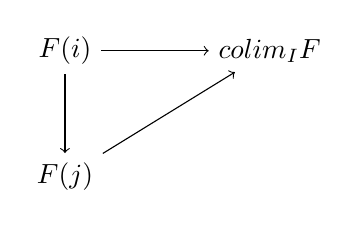
\begin{tikzpicture}
  \node (fi) at (0,0) {$F(i)$};
  \node (c) at (2.6,0) {$\operatorname{colim}_I F$};
  \node (fj) at (0,-1.6) {$F(j)$};
  \draw[->] (fi) -- (c);
  \draw[->] (fi) -- (fj);
  \draw[->] (fj) -- (c);
\end{tikzpicture}
\end{center}
交换。另一方面，由对 $F$ 的假设，三角形
\begin{center}
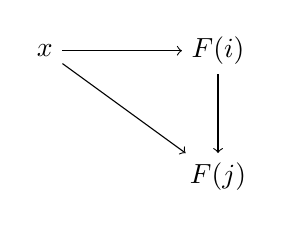
\begin{tikzpicture}
  \node (x) at (0,0) {$x$};
  \node (fi) at (2.2,0) {$F(i)$};
  \node (fj) at (2.2,-1.6) {$F(j)$};
  \draw[->] (x) -- (fi);
  \draw[->] (x) -- (fj);
  \draw[->] (fi) -- (fj);
\end{tikzpicture}
\end{center}
也交换，于是断言得证。

由构造，复合
\[
\operatorname{colim}_{I} F \to
\operatorname{colim}_{I^{\triangleleft}} G \to
\operatorname{colim}_{I} F
\]
是恒等。另一个复合提供一个映射
\[
\operatorname{colim}_{I^{\triangleleft}} G \to
\operatorname{colim}_{I} F \to
\operatorname{colim}_{I^{\triangleleft}} G
\]
其在 $G(j) \to \operatorname{colim}_{I^{\triangleleft}} G$（$j \in I$）上的限制是
典范映射，而其在\trCone{}点上的限制由
$x \to G(i) \to \operatorname{colim}_{I^{\triangleleft}} G$ 给出。这个映射正是
典范映射 $G(\ast) \to \operatorname{colim}_{I^{\triangleleft}} G$，于是上述复合
也是恒等。
\end{proof}

\begin{lemma}\label{lem:join-preserves-colimits}
\trFunctor{} $S \star -$ 与 $- \star S\colon \mathrm{sSet} \to \mathrm{sSet}_{S/}$
保持\trColimit{}。
\end{lemma}

\begin{proof}
只需检验这些\trFunctor{}保持\trCoequalizer{}（coequalizer）——由%
\cref{lem:slice-complete}，它们在 $\mathrm{sSet}$ 中计算——以及保持余积。对于
后者，我们回忆，$\mathrm{sSet}_{S/}$ 中的余积 $(S \to A) \amalg (S \to B)$ 由到
$\mathrm{sSet}$ 中\trPushout{} $S \to A \amalg_S B$ 的典范映射给出（此类\trSlice{}中%
\trColimit{}的描述仍见\cref{lem:slice-complete}）。于是我们观察到
\[
\bigl(S \star \bigl(\coprod_{i \in I} A_i\bigr)\bigr)_n
= S_n \amalg \coprod_{i \in I} (A_i)_n \amalg
\coprod_{k+l=n-1} S_k \times \coprod_{i \in I} (A_i)_l,
\]
而
\[
\coprod_{i \in I} (S \star A_i)_n =
\Bigl. \coprod_{i \in I} \Bigl( S_n \amalg (A_i)_n \amalg
\coprod_{k+l=n-1} S_k \times (A_i)_l \Bigr) \Bigr/ \sim
\]
其中关系把 $\coprod_I S_n$ 与 $S_n$ 等同起来。对于\trCoequalizer{}，陈述由\trJoin{}的\trSimplex{}的显式描述类似地得出。
\end{proof}

\begin{corollary}\label{cor:join-preserves-pushouts}
\trFunctor{} $S \star -$ 与 $- \star S\colon \mathrm{sSet} \to \mathrm{sSet}$
保持\trPushout{}。
\end{corollary}

\begin{proof}
由\cref{lem:join-preserves-colimits}，\trFunctor{} $S \star -$ 与
$- \star S\colon \mathrm{sSet} \to \mathrm{sSet}_{S/}$ 保持所有\trColimit{}，而由
\cref{lem:slice-complete}，\trForgetfulFunctor{}%
$\mathrm{sSet}_{S/} \to \mathrm{sSet}$ 保持\trConnected{}\trColimit{}。由于%
\trPushout{}是\trConnected{}\trColimit{}，断言得证。
\end{proof}

\begin{corollary}\label{cor:slice-join-adjunction}
\trFunctor{} $(p\colon S \to X) \mapsto X_{p/}$ 是
$S \star -\colon \mathrm{sSet} \to \mathrm{sSet}_{S/}$ 的\trRightAdjoint{}。
同样地，\trFunctor{} $(p\colon S \to X) \mapsto X_{/p}$ 是
$- \star S\colon \mathrm{sSet} \to \mathrm{sSet}_{S/}$ 的\trRightAdjoint{}。
\end{corollary}

\begin{proof}
由定义，\trAdjunction{}性质对可表示对象成立。由%
\cref{lem:join-preserves-colimits}，\trFunctor{} $S \star -$ 与 $- \star S$ 保持%
\trColimit{}，于是\trAdjunction{}双射便从可表示对象扩张到所有\trSimplicialSets{}。
\end{proof}

\begin{example*}
设 $\C$ 是一个∞-\trCategory{}，$x \in \C$ 是一个\trObject{}，我们将其视为一个%
\trFunctor{} $x\colon \Delta^0 \to \C$。我们便得到\trSlice{} $\C_{x/}$ 与 $\C_{/x}$。
对一般的\trSimplicialSet{} $K$，我们将记 $K^{\triangleleft} = \Delta^0 \star K$
与 $K^{\triangleright} = K \star \Delta^0$，并称这两个构造为 $K$ 上的\trCone{}（cone）与%
\trCocone{}（cocone）。
\end{example*}

\begin{observation}\label{obs:slice-join-unit-counit}
让我们显式写出\trSlice{}/\trJoin{}\trAdjunction{}的\trUnit{}与\trCounit{}。对固定的\trSimplicialSet{} $S$，该%
\trAdjunction{}的\trCounit{}由如下一个自然映射给出：设 $p\colon S \to X$ 是
$\mathrm{sSet}_{S/}$ 的一个\trObject{}，于是我们得到\trSlice{} $X_{p/}$。那么\trCounit{}是
$\mathrm{sSet}_{S/}$ 中由下式给出的映射 $S \star X_{p/} \to X$：
\[
S_n \amalg \mathrm{Hom}_{\mathrm{sSet}_{S/}}(S \star \Delta^n, X) \amalg
\coprod_{k+l=n-1} S_k \times
\mathrm{Hom}_{\mathrm{sSet}_{S/}}(S \star \Delta^\ell, X) \to X_n,
\]
它在第一个分支上由 $p$ 给出，在第二个分支上由与 $\Delta^n \to S \star \Delta^n$
的预复合诱导，而在最后一个分支上对 $S$ 的每个 $k$-\trSimplex{}由与
$\Delta^k \star \Delta^\ell \to S \star \Delta^\ell$ 的预复合诱导。

同样地，\trUnit{}是映射 $X \to (S \star X)_{\mathrm{can}/}$，其中
$\mathrm{can}\colon S \to S \star X$ 是典范映射。它由把 $X$ 的一个
$n$-\trSimplex{} 与 $S$ 相联而给出，这产生一个映射
\[
X_n \cong \mathrm{Hom}_{\mathrm{sSet}}(\Delta^n, X) \to
\mathrm{Hom}_{\mathrm{sSet}_{S/}}(S \star \Delta^n, S \star X).
\]
\end{observation}

\begin{definition}\label{def:twisted-arrow-category}
设 $\C$ 是一个普通\trCategory{}。我们定义一个新的\trCategory{}%
$\mathrm{Tw}(\C)$，即 $\C$ 的\emph{\trTwistedArrowCategory{}}（twisted arrow
category），如下：\trObject{}是 $\C$ 的\trMorphism{}，而 $\mathrm{Tw}(\C)$ 中从
$f'\colon x' \to y'$ 到 $f\colon x \to y$ 的一个\trMorphism{}由交换图表
\begin{center}
\begin{tikzpicture}
  \node (x) at (0,0) {$x$};
  \node (y) at (2.4,0) {$y$};
  \node (xp) at (0,-1.6) {$x'$};
  \node (yp) at (2.4,-1.6) {$y'$};
  \draw[->] (x) -- node[above] {$f$} (y);
  \draw[->] (xp) -- node[below] {$f'$} (yp);
  \draw[->] (x) -- node[left] {$\alpha$} (xp);
  \draw[->] (yp) -- node[right] {$\beta$} (y);
\end{tikzpicture}
\end{center}
给出。我们也写：序对 $(\alpha, \beta)$ 是从 $f'$ 到 $f = \beta f' \alpha$ 的一个%
\trMorphism{}。复合由把这样的图表拼接在一起而得到。
\end{definition}

\begin{lemma}\label{lem:slice-functorial}
\trSlice{}构造诱导一个\trFunctor{} $\mathrm{Tw}(\mathrm{sSet}) \to \mathrm{sSet}$。
特别地，对于
\[
A \xrightarrow{\ i\ } B \xrightarrow{\ \varphi\ } X
\xrightarrow{\ f\ } Y
\]
存在一个诱导映射
\[
X_{\varphi/} \to X_{\varphi i/} \times_{Y_{f \varphi i/}} Y_{f \varphi/}.
\]
对另一个\trSlice{}同样成立。
\end{lemma}

\begin{proof}
$\mathrm{Tw}(\mathrm{sSet})$ 的\trObject{}由\trSimplicialSets{}的映射
$p\colon S \to X$ 给出，而这样一个\trObject{}被送到 $X_{p/}$\footnote{译注：原书此处作 $X_{/p}$，依证明中的切片记号应为 $X_{p/}$。——译者注}。我们需要阐明这在%
\trTwistedArrowCategory{}的\trMorphism{}上如何是\trFunctor{}性的；也就是说，
我们需要产生一个
典范映射
\[
X_{\varphi/} \to Y_{f \varphi i/},
\]
因为序对 $(i, f)$ 是 $\mathrm{Tw}(\mathrm{sSet})$ 中从 $\varphi$ 到
$f \varphi i$ 的一个\trMorphism{}。

首先，我们构造映射 $X_{\varphi/} \to X_{\varphi i/}$ 与
$X_{\varphi/} \to Y_{f \varphi/}$，它们对应于 $\mathrm{Tw}(\mathrm{sSet})$ 中的%
\trMorphism{}%
\begin{center}
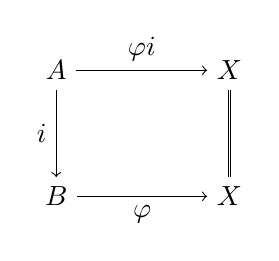
\begin{tikzpicture}
  \node (a) at (0,0) {$A$};
  \node (x) at (2.2,0) {$X$};
  \node (b) at (0,-1.6) {$B$};
  \node (x2) at (2.2,-1.6) {$X$};
  \draw[->] (a) -- node[above] {$\varphi i$} (x);
  \draw[->] (b) -- node[below] {$\varphi$} (x2);
  \draw[->] (a) -- node[left] {$i$} (b);
  \draw[double] (x) -- (x2);
\end{tikzpicture}
\hspace{3.5em}%
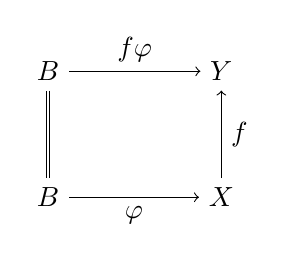
\begin{tikzpicture}
  \node (b) at (0,0) {$B$};
  \node (y) at (2.2,0) {$Y$};
  \node (b2) at (0,-1.6) {$B$};
  \node (x) at (2.2,-1.6) {$X$};
  \draw[->] (b) -- node[above] {$f \varphi$} (y);
  \draw[->] (b2) -- node[below] {$\varphi$} (x);
  \draw[double] (b) -- (b2);
  \draw[->] (x) -- node[right] {$f$} (y);
\end{tikzpicture}
\end{center}
利用这些构造，我们类似地得到映射
\[
X_{\varphi i/} \to Y_{f \varphi i/} \leftarrow Y_{f \varphi/},
\]
然后我们将证明图表
\begin{center}
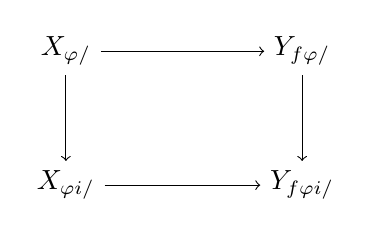
\begin{tikzpicture}
  \node (a) at (0,0) {$X_{\varphi/}$};
  \node (b) at (3,0) {$Y_{f \varphi/}$};
  \node (c) at (0,-1.7) {$X_{\varphi i/}$};
  \node (d) at (3,-1.7) {$Y_{f \varphi i/}$};
  \draw[->] (a) -- (b);
  \draw[->] (a) -- (c);
  \draw[->] (b) -- (d);
  \draw[->] (c) -- (d);
\end{tikzpicture}
\end{center}
交换。这已经是\trTwistedArrowCategory{}中\trFunctor{}性的一部分，因为序对 $(i, f)$ 满足
\[
(i, \mathrm{id}) \circ (\mathrm{id}, f) = (i, f) =
(\mathrm{id}, f) \circ (i, \mathrm{id}),
\]
正如下面两个图表所示：
\begin{center}
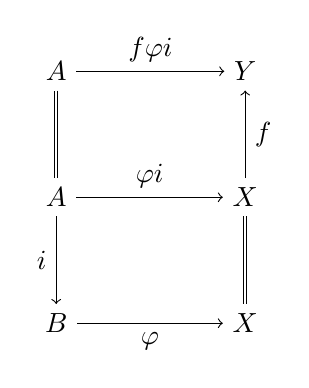
\begin{tikzpicture}
  \node (a1) at (0,0) {$A$};
  \node (y1) at (2.4,0) {$Y$};
  \node (a2) at (0,-1.6) {$A$};
  \node (x2) at (2.4,-1.6) {$X$};
  \node (b3) at (0,-3.2) {$B$};
  \node (x3) at (2.4,-3.2) {$X$};
  \draw[->] (a1) -- node[above] {$f \varphi i$} (y1);
  \draw[->] (a2) -- node[above] {$\varphi i$} (x2);
  \draw[double] (a1) -- (a2);
  \draw[->] (x2) -- node[right] {$f$} (y1);
  \draw[->] (a2) -- node[left] {$i$} (b3);
  \draw[->] (b3) -- node[below] {$\varphi$} (x3);
  \draw[double] (x2) -- (x3);
\end{tikzpicture}
\hspace{3.5em}%
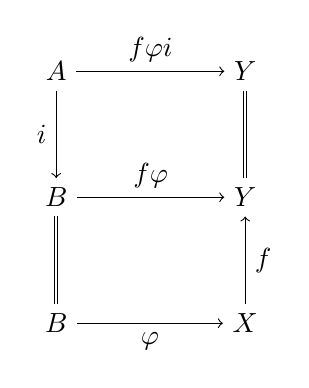
\begin{tikzpicture}
  \node (a1) at (0,0) {$A$};
  \node (y1) at (2.4,0) {$Y$};
  \node (b2) at (0,-1.6) {$B$};
  \node (y2) at (2.4,-1.6) {$Y$};
  \node (b3) at (0,-3.2) {$B$};
  \node (x3) at (2.4,-3.2) {$X$};
  \draw[->] (a1) -- node[above] {$f \varphi i$} (y1);
  \draw[->] (a1) -- node[left] {$i$} (b2);
  \draw[double] (y1) -- (y2);
  \draw[->] (b2) -- node[above] {$f \varphi$} (y2);
  \draw[double] (b2) -- (b3);
  \draw[->] (x3) -- node[right] {$f$} (y2);
  \draw[->] (b3) -- node[below] {$\varphi$} (x3);
\end{tikzpicture}
\end{center}
映射 $X_{\varphi/} \to X_{\varphi i/}$ 在 $A$ 之下\trAdjunction{}于一个映射
$A \star X_{\varphi/} \to X$，我们将其定义为典范复合
\[
A \star X_{\varphi/} \to B \star X_{\varphi/} \to X
\]
它由 $i$ 所诱导的映射与该\trAdjunction{}的\trCounit{}组成。同样地，映射
$X_{\varphi/} \to Y_{f \varphi/}$ 在 $B$ 之下\trAdjunction{}于一个映射
$B \star X_{\varphi/} \to Y$，我们将其定义为复合
\[
B \star X_{\varphi/} \to X \to Y
\]
它由\trCounit{}再接 $f$ 组成。为了看出图表
\begin{center}
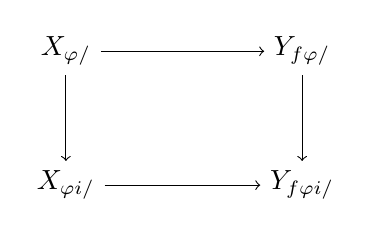
\begin{tikzpicture}
  \node (a) at (0,0) {$X_{\varphi/}$};
  \node (b) at (3,0) {$Y_{f \varphi/}$};
  \node (c) at (0,-1.7) {$X_{\varphi i/}$};
  \node (d) at (3,-1.7) {$Y_{f \varphi i/}$};
  \draw[->] (a) -- (b);
  \draw[->] (a) -- (c);
  \draw[->] (b) -- (d);
  \draw[->] (c) -- (d);
\end{tikzpicture}
\end{center}
交换，我们观察到，两个复合都\trAdjunction{}于映射
\[
A \star X_{\varphi/} \to B \star X_{\varphi/} \to X \to Y.
\]
随后容易看出，这个构造在 $\mathrm{Tw}(\mathrm{sSet})$ 中是\trFunctor{}性的。对于%
另一个\trSlice{}，论证是类似的。
\end{proof}

\begin{lemma}\label{lem:slice-join-lifting}
\trSlice{}/\trJoin{}\trAdjunction{}在形如下述图表的\trLiftingProblem{}与形如下述图表的\trLiftingProblem{}之间
诱导一个双射：
\begin{center}
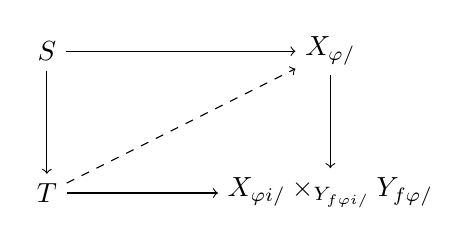
\begin{tikzpicture}
  \node (s) at (0,0) {$S$};
  \node (r) at (3.6,0) {$X_{\varphi/}$};
  \node (l) at (0,-1.8) {$T$};
  \node (b) at (3.6,-1.8) {$X_{\varphi i/} \times_{Y_{f \varphi i/}} Y_{f \varphi/}$};
  \draw[->] (s) -- (r);
  \draw[->] (s) -- (l);
  \draw[->] (l) -- (b);
  \draw[->] (r) -- (b);
  \draw[->, dashed] (l) -- (r);
\end{tikzpicture}
\end{center}
与
\begin{center}
\begin{tikzpicture}
  \node (b0) at (0,0) {$B$};
  \node (m) at (4,0) {$A \star T \amalg_{A \star S} B \star S$};
  \node (x) at (7.6,0) {$X$};
  \node (bt) at (4,-1.8) {$B \star T$};
  \node (y) at (7.6,-1.8) {$Y$};
  \draw[->] (b0) -- (m);
  \draw[->] (m) -- (x);
  \draw[->] (m) -- (bt);
  \draw[->] (bt) -- (y);
  \draw[->] (x) -- (y);
  \draw[->, bend left=35] (b0) to node[above] {$\varphi$} (x);
  \draw[->, dashed] (bt) -- (x);
\end{tikzpicture}
\end{center}
\end{lemma}

\begin{proof}
见\cref{ex:slice-join-lifting-bijection}。
\end{proof}

\cref{lem:box-anodyne} 与\cref{thm:angle-fi-fibration} 的一个类似结论，对联与%
\trSlice{}（代替积\trSimplicialSet{}与 hom \trSimplicialSet{}）成立。

\begin{lemma}\label{lem:join-box-anodyne}
设 $i\colon A \to B$ 与 $g\colon S \to T$ 是\trMonomorphism{}。那么诱导映射
\[
i \hat{\star} g\colon A \star T \amalg_{A \star S} B \star S \to B \star T
\]
是一个\trMonomorphism{}。此外，
\begin{enumerate}[label=(\arabic*)]
  \item 它是\trInnerAnodyne{}的，若 $i$ 是\trRightAnodyne{}的或 $g$ 是\trLeftAnodyne{}的；
  \item 它是\trLeftAnodyne{}的，若 $i$ 是\trLeftAnodyne{}的；
  \item 它是\trRightAnodyne{}的，若 $g$ 是\trRightAnodyne{}的。
\end{enumerate}
\end{lemma}

\begin{proof}
对于 (1)，让我们证明 $i$ 为\trRightAnodyne{}的情形。我们断言：由所有使得映射
$i \hat{\star} g$ 为\trInnerAnodyne{}的（对任意\trMonomorphism{} $g\colon S \to T$）%
\trMonomorphism{} $i\colon A \to B$ 组成之集是一个\trSaturatedClass{}：这是因为它正是由所有
对形如
\[
X_{\varphi/} \to X_{\varphi i/} \times_{Y_{f \varphi i/}} Y_{f \varphi/}
\]
的\trMorphism{}满足 LLP 的\trMonomorphism{}组成的集合，其中 $f\colon X \to Y$
是一个\trInnerFibration{}，而 $\varphi\colon T \to X$ 是任意映射。于是只需证明：
对 $0 < j \le n$，\trHornInclusion{} $\Lambda^n_j \to \Delta^n$ 落在这个集合
之中。至于由所有
使得映射 $(\Lambda^n_j \to \Delta^n) \hat{\star} g$ 为\trInnerAnodyne{}的%
\trMonomorphism{} $g\colon S \to T$ 组成之集也是一个\trSaturatedSet{}，我们把它留作练习。
于是只需讨论 $g$ 为\trBoundaryInclusion{} $\partial \Delta^m \to \Delta^m$ 的
情形。在这种情形，
我们必须检验
\[
\Lambda^n_j \star \Delta^m \cup \Delta^n \star \partial \Delta^m
\to \Delta^n \star \Delta^m
\]
是\trInnerAnodyne{}的。但这由\cref{ex:join-horn-computation} 得出，该练习证明前者由 $\Lambda^{n+1+m}_j$
给出，而由于 $j \le n < n + 1 + m$，它现在是一个内\trHorn{}。

$g$ 为\trLeftAnodyne{}的情形由一个类似的计算得出，它基于这一事实：
\[
\partial \Delta^m \star \Delta^n \cup \Delta^m \star \Lambda^n_j
\to \Delta^{m+1+n}
\]
同构于包含 $\Lambda^{m+1+n}_{m+1+j} \to \Delta^{m+1+n}$，且 $0 \le j < n$，于是这
又是一个内\trHorn{}。

现在让我们证明 (2)。利用与之前相同的归约论证，只需处理
$i\colon \Lambda^n_j \to \Delta^n$（其中 $0 \le j < n$）而
$g\colon \partial \Delta^m \to \Delta^m$ 为\trBoundaryInclusion{}的情形。于是，
如前，我们得到
映射 $i \hat{\star} g$ 由 $\Lambda^{n+1+m}_j \to \Delta^{n+1+m}$（其中
$0 \le j < n$）给出，它显然是一个%
\trLeftAnodyne{}映射。情形 (3) 是类似的。
\end{proof}

\begin{theorem}\label{thm:slice-fibration}
设
\[
A \xrightarrow{\ i\ } B \xrightarrow{\ \varphi\ } X
\xrightarrow{\ f\ } Y
\]
为可复合的映射，并假设 $i$ 是一个\trMonomorphism{}，而 $f$ 是一个%
\trInnerFibration{}。
\begin{enumerate}[label=(\arabic*)]
  \item 诱导映射
\[
X_{\varphi/} \to X_{\varphi i/} \times_{Y_{f \varphi i/}} Y_{f \varphi/}
\]
是一个\trLeftFibration{}。
  \item 若映射 $f\colon X \to Y$ 是一个\trLeftFibration{}，则诱导映射
\[
X_{/\varphi} \to X_{/\varphi i} \times_{Y_{/f \varphi i}} Y_{/f \varphi}
\]
是一个\trLeftFibration{}。
  \item 若映射 $i\colon A \to B$ 是\trRightAnodyne{}的，则映射
\[
X_{\varphi/} \to X_{\varphi i/} \times_{Y_{f \varphi i/}} Y_{f \varphi/}
\]
是一个\trTrivialFibration{}。
  \item 若映射 $f\colon X \to Y$ 是一个\trTrivialFibration{}，则映射
\[
X_{\varphi/} \to X_{\varphi i/} \times_{Y_{f \varphi i/}} Y_{f \varphi/}
\]
是一个\trTrivialFibration{}。
\end{enumerate}
\end{theorem}

\begin{proof}
我们再次考虑一个一般的\trLiftingProblem{}%
\begin{center}
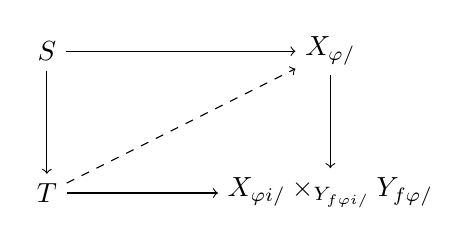
\begin{tikzpicture}
  \node (s) at (0,0) {$S$};
  \node (r) at (3.6,0) {$X_{\varphi/}$};
  \node (l) at (0,-1.8) {$T$};
  \node (b) at (3.6,-1.8) {$X_{\varphi i/} \times_{Y_{f \varphi i/}} Y_{f \varphi/}$};
  \draw[->] (s) -- (r);
  \draw[->] (s) -- (l);
  \draw[->] (l) -- (b);
  \draw[->] (r) -- (b);
  \draw[->, dashed] (l) -- (r);
\end{tikzpicture}
\end{center}
这个\trLiftingProblem{}（由\cref{lem:slice-join-lifting}，或者更确切地说由\cref{ex:slice-join-lifting-bijection}）等价于
下述\trLiftingProblem{}：
\begin{center}
\begin{tikzpicture}
  \node (b0) at (0,0) {$B$};
  \node (m) at (4,0) {$A \star T \amalg_{A \star S} B \star S$};
  \node (x) at (7.6,0) {$X$};
  \node (bt) at (4,-1.8) {$B \star T$};
  \node (y) at (7.6,-1.8) {$Y$};
  \draw[->] (b0) -- (m);
  \draw[->] (m) -- (x);
  \draw[->] (m) -- (bt);
  \draw[->] (bt) -- (y);
  \draw[->] (x) -- (y);
  \draw[->, bend left=35] (b0) to node[above] {$\varphi$} (x);
  \draw[->, dashed] (bt) -- (x);
\end{tikzpicture}
\end{center}
为了证明 (1)，我们于是需要检验：只要 $S \to T$ 是\trLeftAnodyne{}的，左边的竖直映射就是%
\trInnerAnodyne{}的。但这由\cref{lem:join-box-anodyne} 第 (1) 部分得出。为了证明
(2)，我们需要检验：只要映射 $S \to T$ 是\trLeftAnodyne{}的，映射
\[
S \star B \amalg_{S \star A} T \star A \to T \star B
\]
就是\trLeftAnodyne{}的。但这正是\cref{lem:join-box-anodyne} 第 (2) 部分的内容。为了证明
(3)，我们观察到：若 $S \to T$ 是一个\trMonomorphism{}而 $A \to B$ 是\trRightAnodyne{}的，
则映射 $A \star T \amalg_{A \star S} B \star S \to B \star T$ 是\trInnerAnodyne{}的，
这仍由\cref{lem:join-box-anodyne} 第 (1) 部分得出。最后，为了证明 (4)，我们只需
利用如下事实：映射 $A \star T \amalg_{A \star S} B \star S \to B \star T$ 总是一个%
\trMonomorphism{}，而\trTrivialFibration{}对\trMonomorphism{}满足 RLP。
\end{proof}

让我们在下面的推论中写出一些显式的特殊情形。

\begin{corollary}\label{cor:slice-special-cases}
设给定与之前一样的映射 $A \to B \to X \to Y$，其中 $A \to B$ 是一个%
\trMonomorphism{}，而 $X \to Y$ 是一个\trInnerFibration{}。
\begin{enumerate}[label=(\arabic*)]
  \item 若 $Y = \ast$（从而 $X$ 是一个∞-\trCategory{}），我们得到
  $X_{\varphi/} \to X_{\varphi i/}$ 是一个\trLeftFibration{}，而
  $X_{/\varphi} \to X_{/\varphi i}$ 是一个\trRightFibration{}。特别地，若
  $A = \varnothing$，则映射 $X_{\varphi/} \to X$ 是一个\trLeftFibration{}，而
  $X_{/\varphi} \to X$ 是一个\trRightFibration{}。进而，若 $X$ 是∞-\trCategory{}，
  则 $X_{\varphi/}$ 与 $X_{/\varphi}$ 也是。
  \item 若 $Y = \ast$（从而 $X$ 是一个∞-\trCategory{}），我们得到：
  $X_{\varphi/} \to X_{\varphi i/}$ 是一个\trTrivialFibration{}，若 $A \to B$ 是%
  \trRightAnodyne{}的；而 $X_{/\varphi} \to X_{/\varphi i}$ 是一个\trTrivialFibration{}，若
  $A \to B$ 是\trLeftAnodyne{}的。
  \item 若 $f\colon X \to Y$ 是一个\trTrivialFibration{}，考虑 $A = \varnothing$
  的情形。那么映射 $X_{\varphi/} \to X \times_Y Y_{f \varphi/}$ 是一个%
  \trTrivialFibration{}。此外，映射 $X \times_Y Y_{f \varphi/} \to Y_{f \varphi/}$
  是 $X \to Y$ 的一个\trPullback{}，因而也是一个\trTrivialFibration{}。
\end{enumerate}
\end{corollary}

这一结果的又一个特殊情形如下：设 $\C$ 是一个∞-\trCategory{}，而
$f\colon x \to y$ 是 $\C$ 中的一个\trMorphism{}。我们可以考虑情形
\[
\Delta^0 \to \Delta^1 \to \C \to \ast
\]
并得到映射
\[
\C_{/x} \leftarrow \C_{/f} \to \C_{/y}
\]
它们对应于 $f$ 到 $\Delta^0$ 的两个限制（对另一个\trSlice{}同样如此）。由于包含
$\{0\} \to \Delta^1$ 是\trLeftAnodyne{}的，由\cref{cor:slice-special-cases} 第 (2) 部分
得出，映射 $\C_{/f} \to \C_{/x}$ 是一个\trTrivialFibration{}。因此，我们可以选取
一个\trSectionMap{}，从而得到复合
\[
\C_{/x} \to \C_{/f} \to \C_{/y},
\]
我们可以非正式地把它想作与 $f$ 作后合成的那个\trFunctor{}。对另一个\trSlice{}施行同样
的操作，便得到一个\trFunctor{} $\C_{y/} \to \C_{x/}$，我们可以把它想作与 $f$ 作
预合成。
